\documentclass[9pt,conference,a4paper]{IEEEtran}
\IEEEoverridecommandlockouts

\usepackage{graphicx}
\usepackage{floatrow}
\usepackage{amsmath}

\title{Deconvolution enhanced Generalized Q-Sampling 2 \\ and DSI deconvolution}
\author{
	\IEEEauthorblockN{
		Eleftherios Garyfallidis\IEEEauthorrefmark{1},
		Michael Paquette\IEEEauthorrefmark{1},
		Samuel St-Jean\IEEEauthorrefmark{1},
		Pierrick Coup\'e\IEEEauthorrefmark{2},
		Maxime Descoteaux\IEEEauthorrefmark{1}
	}

	\IEEEauthorblockA{\IEEEauthorrefmark{1} Sherbrooke Connectivity Imaging Lab (SCIL), Computer Science department, Universit\'e de Sherbrooke, Sherbrooke, Canada}
	\IEEEauthorblockA{\IEEEauthorrefmark{2} CNRS, Laboratoire Bordelais de Recherche en Informatique, Bordeaux, France}
}

\begin{document}
\maketitle

For the purpose of the ISBI HARDI reconstruction challenge 2013 and for the heavyweight category, we reconstructed the diffusion datasets using two methods: a) Generalized Q-sampling Imaging 2 \cite{Garyfallidis_thesis}, \cite{yeh-etal:10} with spherical deconvolution \cite{descoteaux-deriche-etal:09},\cite{Descoteaux2008} (GQID),  and b) Diffusion Spectrum Imaging with Deconvolution \cite{canales-rodriguez-etal:10} (DSID).

GQI2 provides a direct analytical formula to calculate the solid angle ODF ($\psi_{GQI2}$) of DSI without the need to first estimate the diffusion propagator:
\begin{equation}
\psi_{GQI2}(\mathbf{u}) = \lambda^{3}\int S(\mathbf{q})H(2\pi\lambda\mathbf{q}\cdot\mathbf{u})d\mathbf{q}
\end{equation}
\noindent where $\mathbf{u}$ is the unit direction in the sphere, $\mathbf{q}$ is the q-space wave vector, $S$ is the DW signal, $\lambda$ is a smoothing parameter called the sampling length and  \\
\begin{equation*}
H(x)=\begin{cases}
2\cos(x)/ x^{2} + (x^{2}-2)\sin(x)/ x^{3},\qquad x\neq0\\
\qquad\qquad 1/3 \qquad\qquad\qquad\qquad \;\;,\qquad x=0
\end{cases}
\end{equation*}

In \cite{Garyfallidis_thesis}, it was shown that $\psi_{GQI2}$ creates ODFs with higher angular accuracy than standard DSI ODFs. In this work, we further extended $\psi_{GQI2}$ with the spherical deconvolution transform (SDT).

The SDT is a sharpening operation which transforms the smooth diffusion ODF into a sharper fiber ODF \cite{tournier-calamante-etal:07}. The idea here is that an ODF for example the GQI2 ODF $\psi_{GQI2}$ can be formed by convolution between the single fiber diffusion ODF kernel, $R$ and the true fiber ODF $\psi_{GQID}$
\begin{equation}
\psi_{GQI2}(\mathbf{u})=\displaystyle\int_{|w|=1} R(\mathbf{u} \cdot \mathbf{w}) \psi_{GQID}(\mathbf{w}) dw\label{eq:Conv}
\end{equation}
The deconvolution is a fast converging iterative process. 

In order to deal with the high levels of noise, the diffusion weighted (DW) datasets for SNR 10 and 20 were denoised with adapted non-local means filtering \cite{descoteaux-wiest-daessle-etal:08} using a rician noise model. As proposed in \cite{descoteaux-wiest-daessle-etal:08}, each DW images were processed independently.The DW dataset with SNR 30 was left intact and no further denoising was performed.

In GQI2, we usually use $2\le\lambda\le3$  as higher values can give noisier ODFs as we see at Fig.1Left. However, higher values of $\lambda$ have the advantage that we are sampling from a higher radius in q-space (higher b-values) where most of the angular information lives. Using the GQID, we show at Fig.1Right that we can eliminate those noisy peaks and obtain sharper ODFs.

\begin{figure}[h]
\begin{centering}
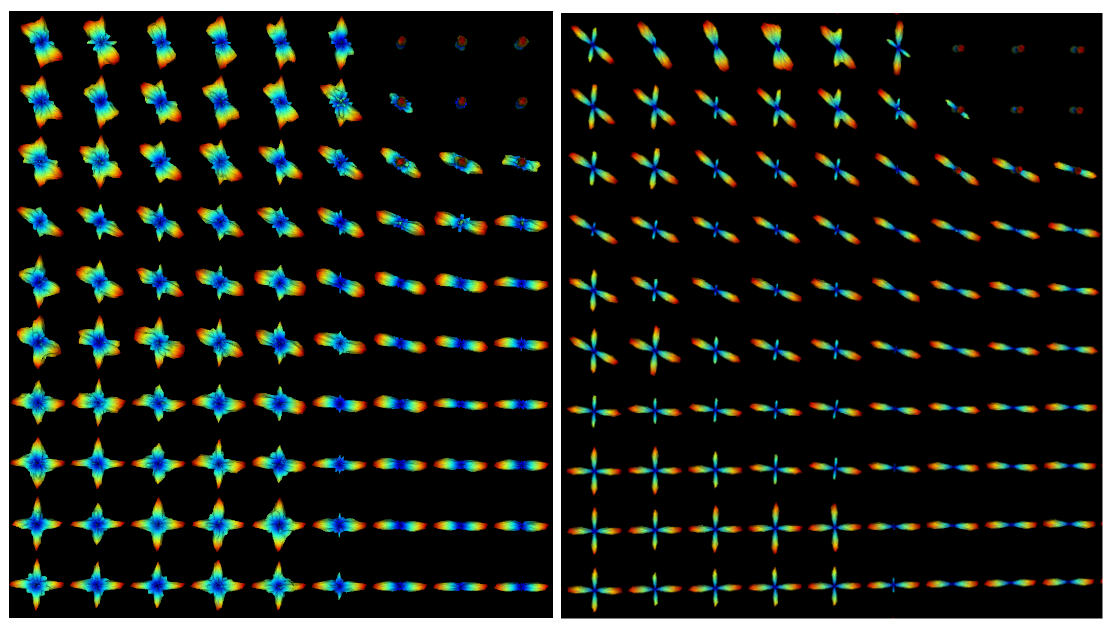
\includegraphics[scale=.9]{gqi2_vs_gqid_snr30}
\end{centering}
\caption{A detail of slice Y=22 from the test data of the HARDI reconstruction challenge 2013 with GQI2 on the left and GQID ODFs on the right.}
\end{figure}

Apart from the GQID, for comparisons we also performed reconstructions using DSI with deconvolution \cite{canales-rodriguez-etal:10}. This deconvolution is not a spherical one, but it is performed in the 3D grid of the DSI propagator using Lucy-Richardson deconvolution. DSID is known to create very sharp ODFs from last year's ISBI challenge.

% \begin{figure}[h]
% \begin{centering}
% \includegraphics[scale=1.]{dsid_snr_30}
% \end{centering}
% \caption{A detail of slice Y=22 from the test data of the HARDI reconstruction challenge 2013 with DSID ODFs.}
% \end{figure}

In order to find the best parameters for the methods described here, we created a connectivity matrix after generating deterministic streamlines from the ODFs of the training set using the method provided by \cite{Girard2012a}. We finally selected the parameters which minimized the number of missing and false bundles in the training set and used those with the test datasets. For DSID we used a propagator grid of $35\times35\times35$. For GQID we used sampling length of $\lambda=3.5$, SDT ratio of $0.22$ and spherical harmonic order of 8. For the challenge we submitted all results with ODFs saved as spherical harmonic coefficients of order 8. The source code for the methods described in this paper is available at dipy.org.
\bibliographystyle{ieeetr}
\bibliography{/home/eleftherios/Documents/scil-bibtex/scilBibTex}

\end{document}


